\section{Methodology}
\label{sec:motion-capture-data-methodology}

We utilize files from the CMU Motion Capture Library \cite{CarnegieMellonUniversity}, specifically XX.asf files and XX\_YY.amc files, where XX represents the subject (describing the skeleton or body of the performer) and YY represents the motion (the action performed). In Figure \ref{fig:skeleton}, we illustrate the skeleton structure, while Figure \ref{fig:jump_motion} shows a visual representation of a jump motion, combining the motion data with the skeleton structure.

Our study focuses on 44 motions, as listed in Table \ref{tab:shape_analysis_movements}: 9 'forward jumps', 9 'runs/jogs', 10 'walks', 9 'boxing' sequences, and 7 'stair climbing' sequences. These motions were chosen due to the availability of sufficient AMC files for each category. Each motion consists of 131 frames, matching the typical duration of a 'forward jump' motion, and all are recorded at a frame rate of 120 Hz. We ensured that the defining part of each motion was clearly visible, such as observing a punch in the boxing sequences.

The dataset includes ASF (Actor Skeleton File) and AMC (Actor Motion Capture Data) files. ASF files describe the skeleton structure and establish a base pose, while AMC files capture dynamic motion over time. We convert this data into joint-specific matrices, focusing on 23 joints to reduce noise from smaller joints such as thumbs, toes, and fingers. Each matrix contains rotational data for each timestep, resulting in a format of \((131, 23, 3, 3)\) representing (timestep, joint, rotation matrix).

Our hypothesis is that motions perceived as similar by humans (e.g., walking) are also mathematically similar, despite individual variations. To test this hypothesis, we will categorize the motions into five distinct groups and evaluate if our shape analysis framework accurately captures these similarities.

\begin{figure}[ht]
    \centering
    \begin{subfigure}[b]{0.4\textwidth}
        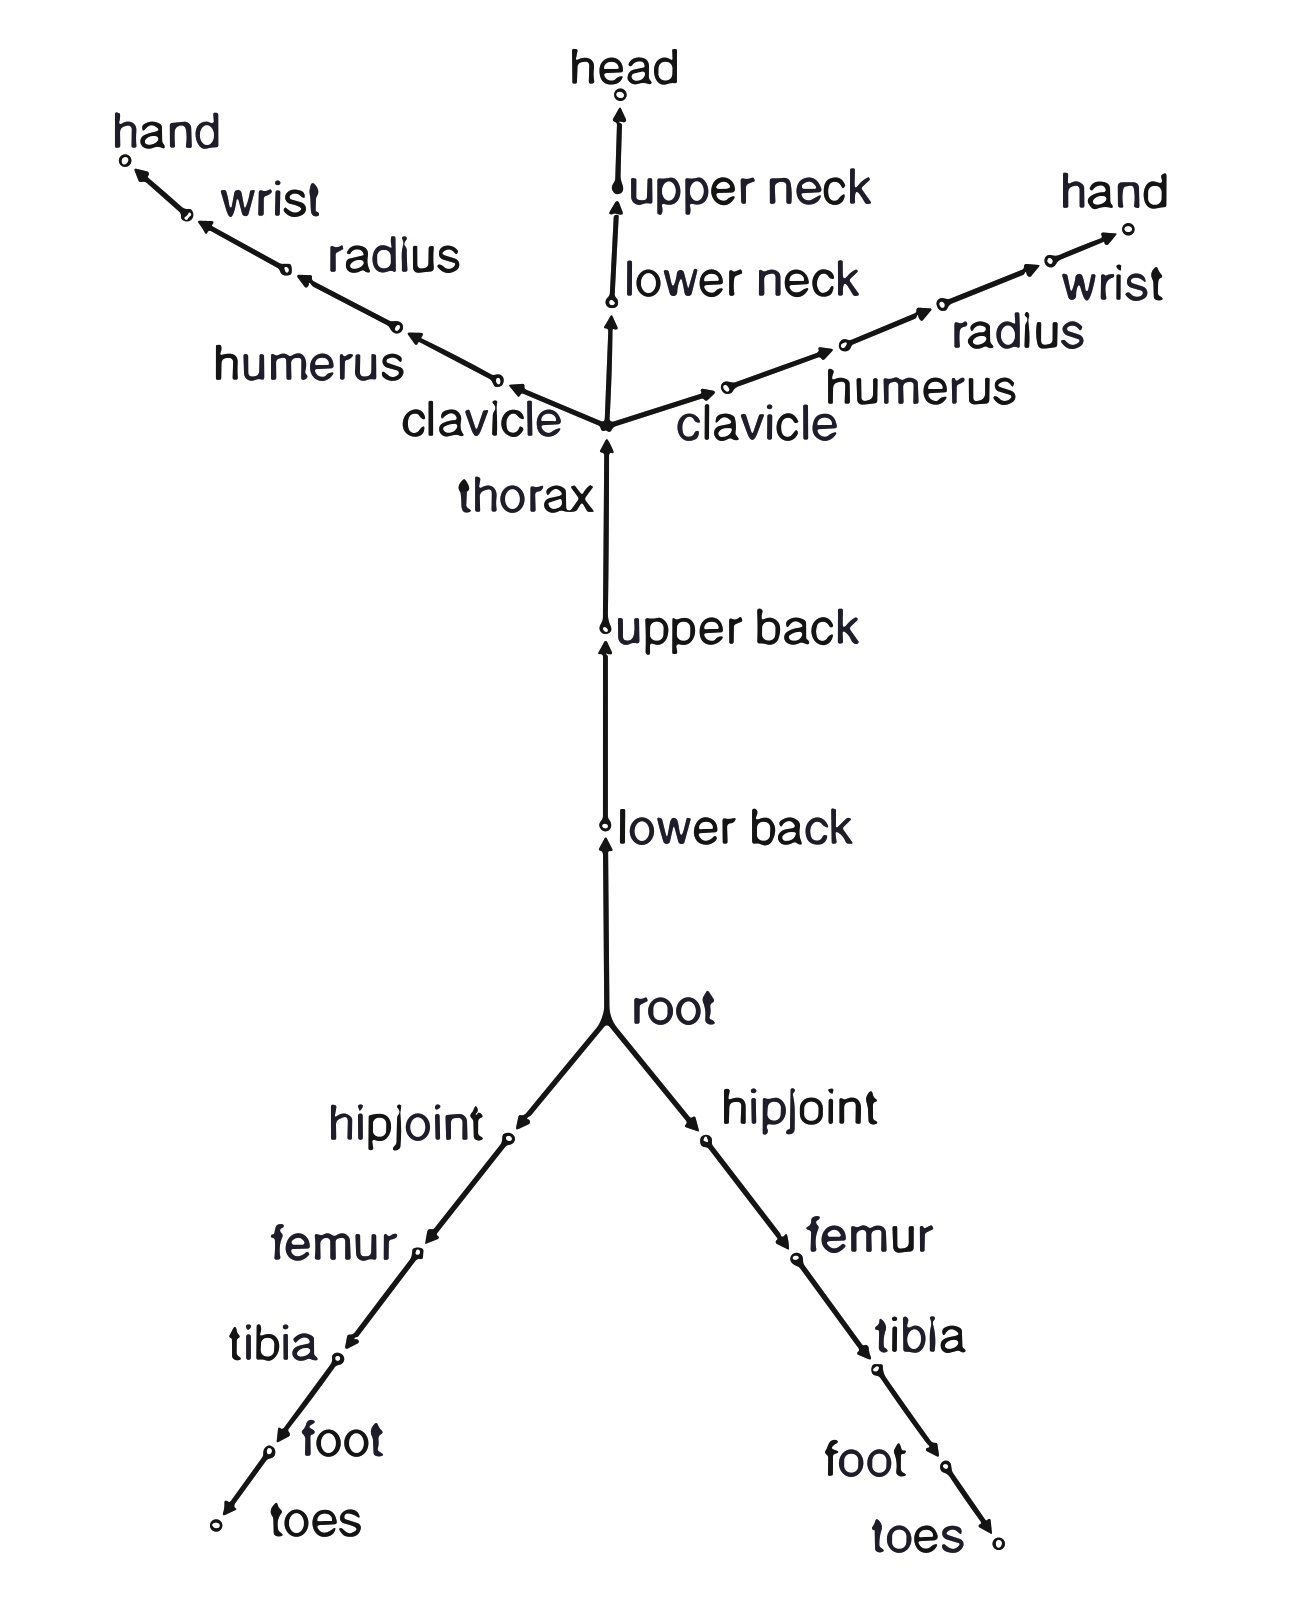
\includegraphics[width=\textwidth]{figures/motion-capture-data/Skeleton_image.png}
        \caption{}
        \label{fig:skeleton}
    \end{subfigure}
    \hfill
    \begin{subfigure}[b]{0.4\textwidth}
        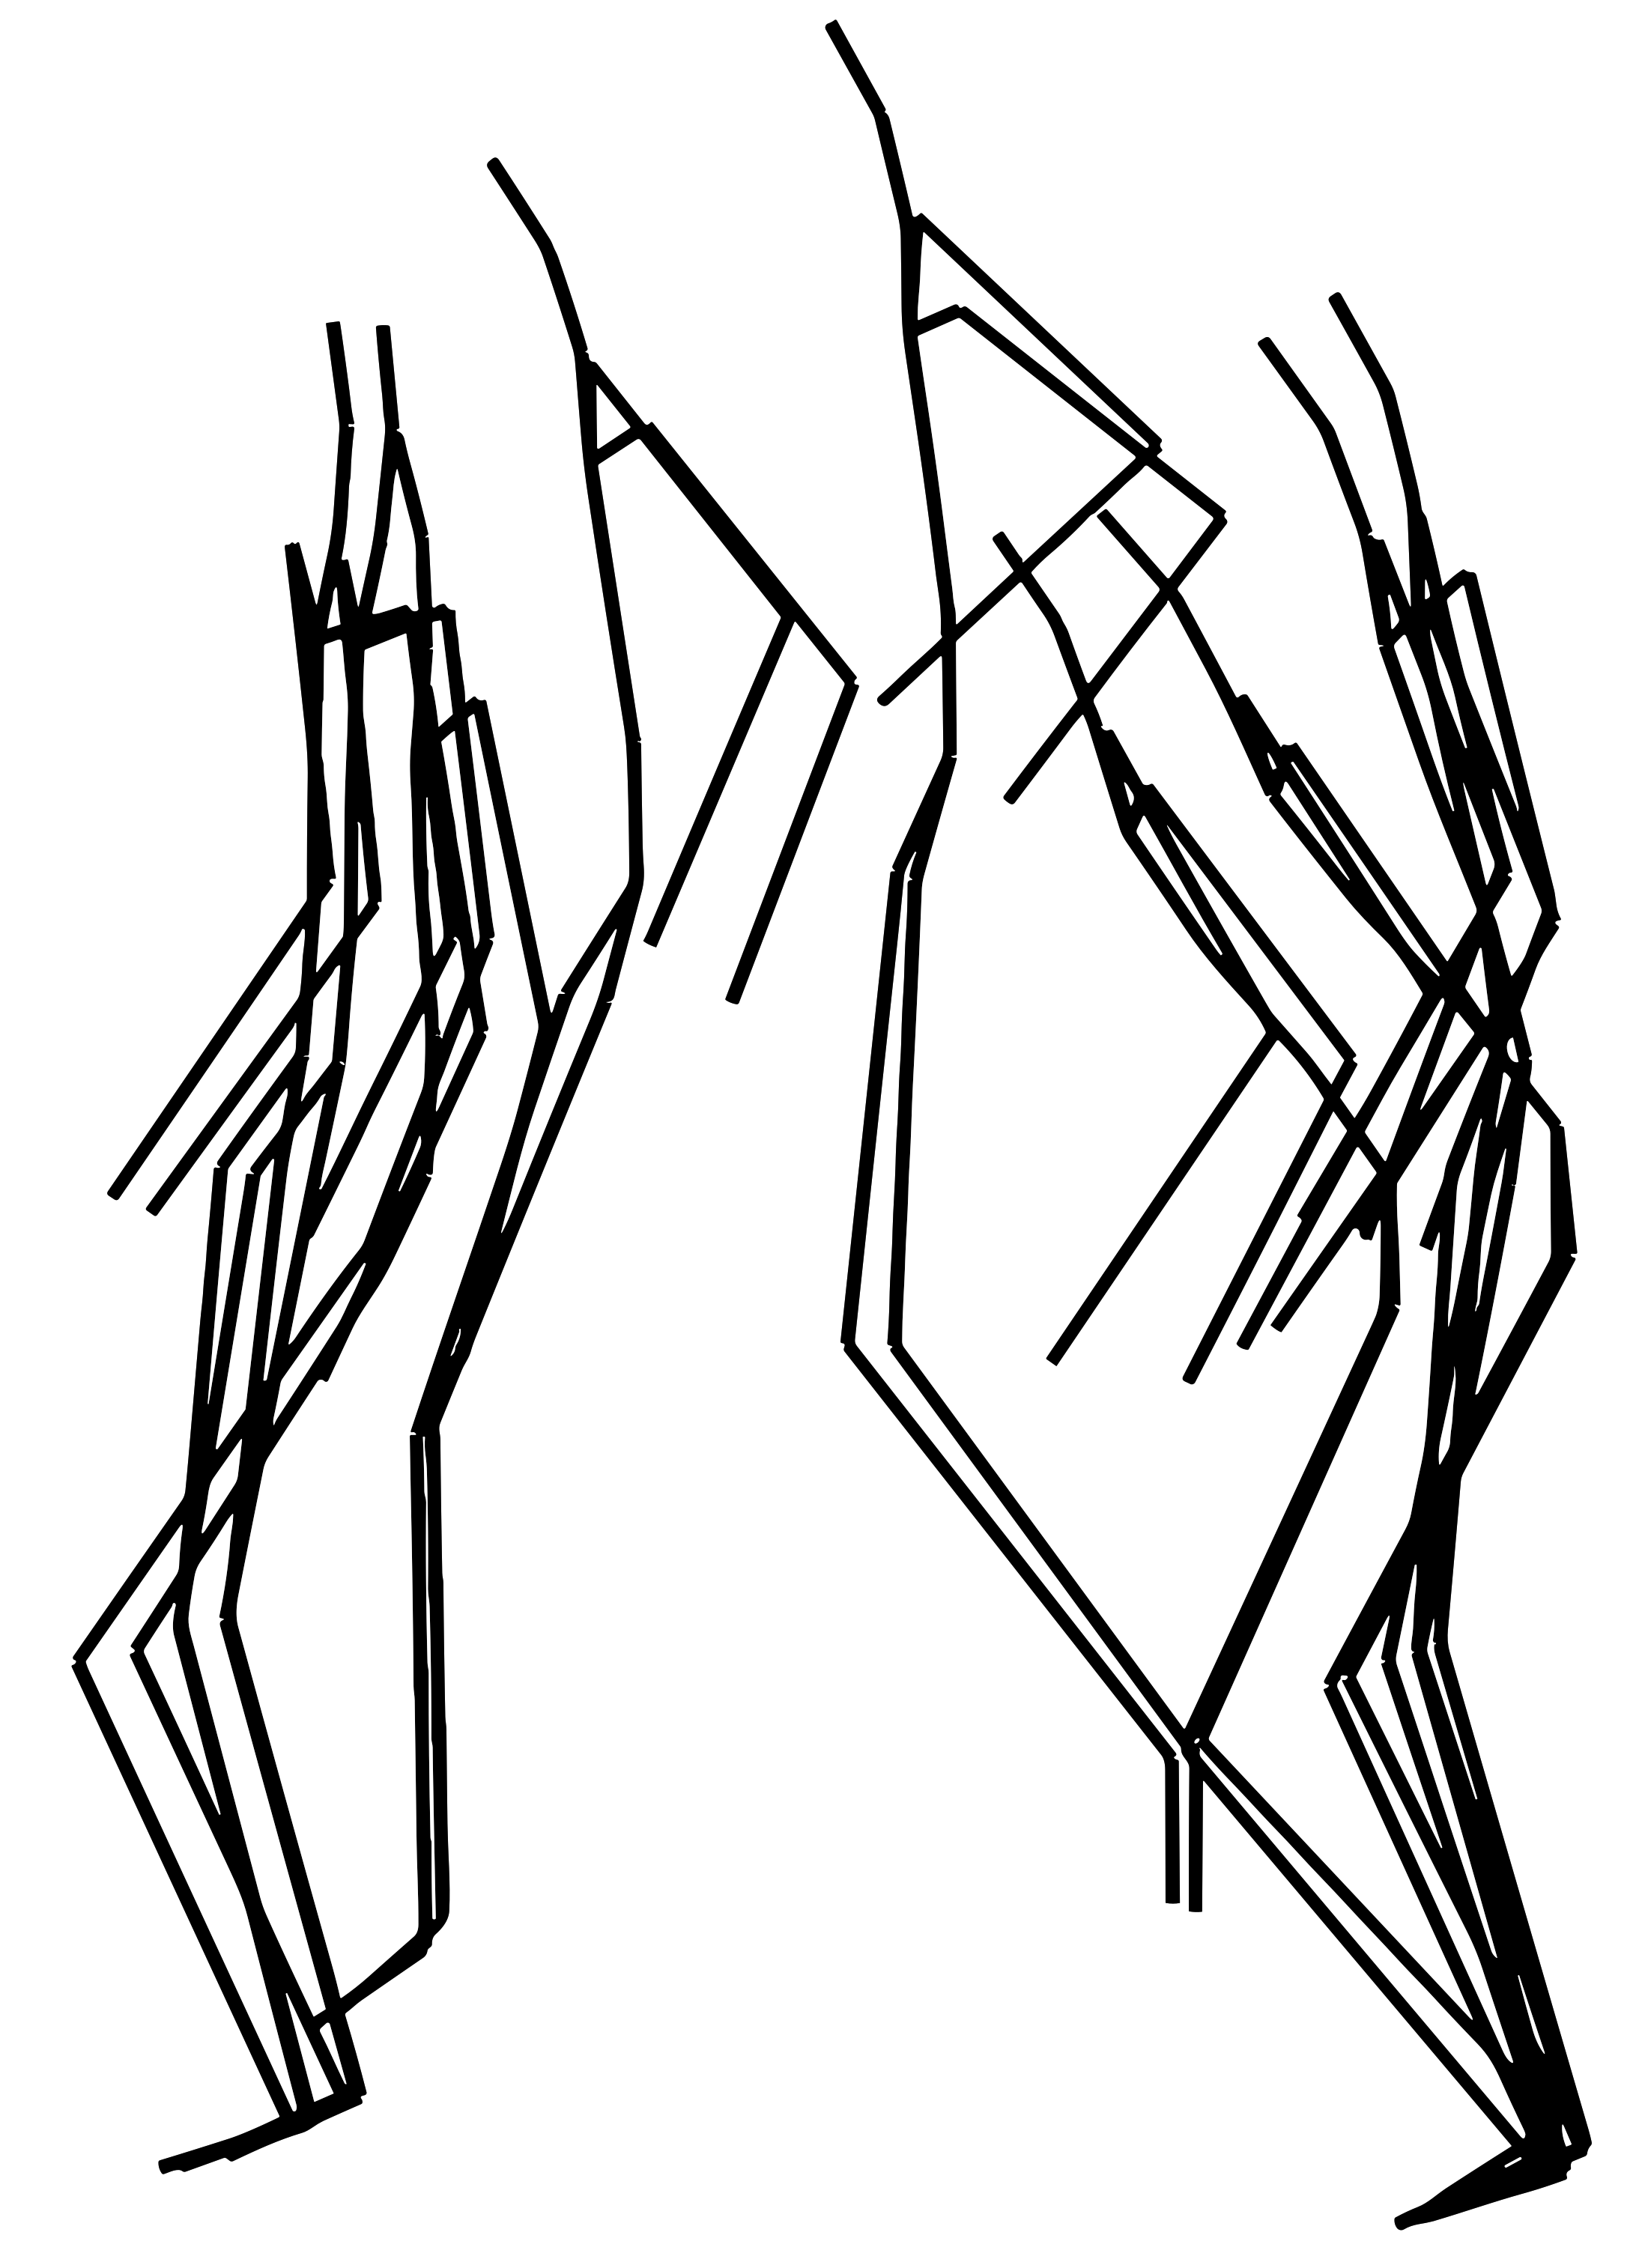
\includegraphics[height=0.3\textheight ,width=0.9\textwidth]{figures/motion-capture-data/Fig_16_05_trace_9_frames.png}
        \caption{}
        \label{fig:jump_motion}
    \end{subfigure}
    \caption[Visualization of the Motion Capture Data]{(a) Illustration of a human skeleton model for computer animation, showing the joint structure with labeled points. Adapted from \cite{bauerLandmarkGuidedElasticShape2015}. (b) Illustration of subject 16 motion 05, depicting one jump motion, 9 timeframes. Data for both illustrations from the CMU Graphics Lab Motion Capture Database \cite{CarnegieMellonUniversity}.}
    \label{fig:combined-motion-capture-figure}
\end{figure}
